% This is "sig-alternate.tex" V1.9 April 2009
% This file should be compiled with V2.4 of "sig-alternate.cls" April 2009
%
% This example file demonstrates the use of the 'sig-alternate.cls'
% V2.4 LaTeX2e document class file. It is for those submitting
% articles to ACM Conference Proceedings WHO DO NOT WISH TO
% STRICTLY ADHERE TO THE SIGS (PUBS-BOARD-ENDORSED) STYLE.
% The 'sig-alternate.cls' file will produce a similar-looking,
% albeit, 'tighter' paper resulting in, invariably, fewer pages.
%
% ----------------------------------------------------------------------------------------------------------------
% This .tex file (and associated .cls V2.4) produces:
%       1) The Permission Statement
%       2) The Conference (location) Info information
%       3) The Copyright Line with ACM data
%       4) NO page numbers
%
% as against the acm_proc_article-sp.cls file which
% DOES NOT produce 1) thru' 3) above.
%
% Using 'sig-alternate.cls' you have control, however, from within
% the source .tex file, over both the CopyrightYear
% (defaulted to 200X) and the ACM Copyright Data
% (defaulted to X-XXXXX-XX-X/XX/XX).
% e.g.
% \CopyrightYear{2007} will cause 2007 to appear in the copyright line.
% \crdata{0-12345-67-8/90/12} will cause 0-12345-67-8/90/12 to appear in the copyright line.
%
% ---------------------------------------------------------------------------------------------------------------
% This .tex source is an example which *does* use
% the .bib file (from which the .bbl file % is produced).
% REMEMBER HOWEVER: After having produced the .bbl file,
% and prior to final submission, you *NEED* to 'insert'
% your .bbl file into your source .tex file so as to provide
% ONE 'self-contained' source file.
%
% ================= IF YOU HAVE QUESTIONS =======================
% Questions regarding the SIGS styles, SIGS policies and
% procedures, Conferences etc. should be sent to
% Adrienne Griscti (griscti@acm.org)
%
% Technical questions _only_ to
% Gerald Murray (murray@hq.acm.org)
% ===============================================================
%
% For tracking purposes - this is V1.9 - April 2009

\documentclass{sig-alternate}
\usepackage{graphicx}
\usepackage[table]{xcolor}
\usepackage{hyperref} %http://www.tug.org/applications/hyperref/manual.html
%\usepackage[usenames,dvipsnames]{color}

%\graphicspath{{./img/}}
%\graphicspath{{../img/}}

\begin{document}
%
% --- Author Metadata here ---
\conferenceinfo{iiWAS2010,}{8-10 November, 2010, Paris, France.}
\CopyrightYear{2010} % Allows default copyright year (20XX) to be over-ridden - IF NEED BE.
\crdata{978-1-4503-0421-4/10/11}  % Allows default copyright data (0-89791-88-6/97/05) to be over-ridden - IF NEED BE.

% --- End of Author Metadata ---


%\title{{\ttlit Morpheus}: An Ontology-based Question Answering System}
\title{{\ttlit Morpheus}: A Deep Web Question Answering System}

%\titlenote{A full version of this paper is available as
%\textit{Author's Guide to Preparing ACM SIG Proceedings Using
%\LaTeX$2_\epsilon$\ and BibTeX} at
%\texttt{www.acm.org/eaddress.htm}}}
%
% You need the command \numberofauthors to handle the 'placement
% and alignment' of the authors beneath the title.
%
% For aesthetic reasons, we recommend 'three authors at a time'
% i.e. three 'name/affiliation blocks' be placed beneath the title.
%
% NOTE: You are NOT restricted in how many 'rows' of
% "name/affiliations" may appear. We just ask that you restrict
% the number of 'columns' to three.
%
% Because of the available 'opening page real-estate'
% we ask you to refrain from putting more than six authors
% (two rows with three columns) beneath the article title.
% More than six makes the first-page appear very cluttered indeed.
%
% Use the \alignauthor commands to handle the names
% and affiliations for an 'aesthetic maximum' of six authors.
% Add names, affiliations, addresses for
% the seventh etc. author(s) as the argument for the
% \additionalauthors command.
% These 'additional authors' will be output/set for you
% without further effort on your part as the last section in
% the body of your article BEFORE References or any Appendices.

\numberofauthors{1} 
\author{
	 \alignauthor Christan Grant, Clint P. George, Joir-dan Gumbs, Joseph N. Wilson, Peter J. Dobbins \\
	 \affaddr{University of Florida, Dept. of Computer Science} \\ \affaddr
{ Gainesville, Florida, USA} \\
\email{\{cgrant, cgeorge, jgumbs, jnw, pjd\} @cise.ufl.edu}
}

\date{2 July 2010}


\maketitle

% Abstract 
\begin{abstract}

The Morpheus question answering system uses deep web search to answer user queries. Queries are represented by a semi-structured format that contains query terms and referenced classes within a specific ontology. Morpheus answers questions by using methods stored in prior successful searches answering similar queries. We rank stored methods based on a similarity measure defined on assigned classes of queries. This measure depends on class heterarchy in a realm-based ontology and the associated text corpora. Finally, we revisit the prior search pathways of the stored searches to construct possible answers. The realm-based ontologies are created using the Wikipedia pages, associated categories, and the synset heterarchy of WordNet. This paper describes the entire process with emphasis on the matching of user queries to stored answering methods.


\end{abstract}


% A category with the (minimum) three required fields
%\category{H.4}{Information Systems Applications}{Miscellaneous}

% A category including the fourth, optional field follows...
%\category{D.2.8}{Software Engineering}{Metrics}[complexity measures, performance measures]

%\category{H.3.3}{Information Search and Retrieval}{Query formulation, Search process}
\category{H.3.4}{Systems and Software}{Question-answering (fact retrieval) systems}
%\category{I.2.6}{Learning}{Concept learning}[Parameter Learning]
%\category{I.2.7}{Natural Language Processing}{Language parsing and understanding, Text analysis}


% \terms{Experimentation, Theory}

\keywords{Federated question answering, Deep web, Ontology creation, Natural language processing, Semantic query matching}


% Introduction 
\section{Introduction}

% Outline 
% ---------------------

% 1. Motivation 
% 2. What are we proposing?  
% 3. Challenges
% 		3.1 User query processing 
% 		3.1 Need of an ontology 
% 4. Realm based question answering 
% 5. About the paper structure 

When traveling though a jungle to a destination, it is easy to get lost.  The first person to journey somewhere may make a number of mistakes when trying to find the best path to their destination. Those who come later find it easier to reach the destination if a well-marked trail has been created. Olsen and Malizia describe this idea as \emph{exploiting trails} \cite{5379671}.  Rather than treating a user's discovery experience as a unique entity, one can exploit the fact that a similar search may have already been performed.  In one study, almost 40 percent of all queries were repetitions of previous queries \cite{1277770}. Thus, reuse of prior searches is one way to optimize the search
process.  Morpheus is a question answering system motivated by reuse of prior web search pathways to yield an answer to a user query. Morpheus follows path-finders to their destinations and not only marks the trail, but also provides a taxi service to take followers to similar
destinations.

There are two distinct Morpheus user roles. A
\textit{path-finder} enters queries in the Morpheus web interface and
searches for an answer to the query using an instrumented web browser. 
This web tracking tool stores the query
and necessary information to revisit the pathways to the page where the path-finder 
found the answer. A \textit{path-follower} uses the Morpheus system much like a regular search engine with a natural language interface. The path-follower enters a question in a text box and receives a guided path to the answer. The system exploits previously found paths to provide an answer.

Morpheus represents user-query details in a semi-structured query (SSQ). It assumes the terms belong to classes of a \textit{consistent} realm-based ontology, that is, one having a singly rooted heterarchy whose subclass/superclass relations have meaningful semantic interpretations. When a path-follower enters a query, Morpheus ranks SSQs in the store based on class similarity. Suppose a regular user asks -\textit{ a 1997 Toyota Camry V6 needs what size tires?} In this query the classes associated with terms, e.g. \emph{Manufacturer} with \emph{Toyota}, helps us identify similar queries.


This paper discusses related question answering and ontology generation systems in section \ref{sec:relatedwork}. Section \ref{sec:systemarch} explains the Morpheus system and its implementation. In Section \ref{sec:results} we describe the current results of our approach.  Finally, we conclude with future goals for the system.


% Related Work 
\section{Related Work}

1. QA systems 
2. Ontology generators 
3. NLP interfaces 


% System arch.
\section{System Architecure}
\label{sec:systemarch}

% This was corrected in my version... (Joir-dan performing diff 2010-06-30)
This section presents ontology and corpora, query processing, ranking queries, and query executing.

\subsection{Using Ontology and Corpora} 
\label{sec:ontology_corpora}

Morpheus uses an ontology that contains categories of a particular realm of interest. Every leaf node in the ontology is associated with a corpus of words belonging to a category.  For example, we have constructed an automotive ontology containing categories relevant to the automotive realm. This ontology provides a structure for reference in the following sections.

%% Comment made by Joir-dan (2010-06-29)
 %%Need to remove any references to Markov Blanket... since we abandoned that ship a while ago... 

Morpheus uses the DBpedia categories, Wikipedia pages and the WordNet synset heterarchy to construct ontologies. This approach is motivated by YAGO \cite{Suchanek2009phd}. First a realm is mapped to a DBpedia category \cite{Bizer2009}. 
Then a \emph{Markov Blanket} \cite{PRIS} is created covering all neighboring categories and using the DBpedia ontology properties \emph{broader} and \emph{narrower}. From here, the system recursively includes all categories up to the root.  

%% ^^^ Needs to remove references to blanket

Once we have the categories belonging to a particular realm, we associate them with WordNet synsets using an approach similar to YAGO\cite{Suchanek2009phd}. We determine a \emph{head noun} in the category name and search for it in the WordNet synsets. DBpedia categories having no WordNet synset match are excluded from our ontology. 

To build a corpus for each of the leaf nodes in the ontology, 
we extract \emph{terms} from the Wikipedia pages associated with the 
the DBpedia categories. From this term corpus, 
we can find the likelihood of a term belonging to a particular category. This assists in categorizing terms in a \emph{path-follower} query.
The likelihood is determined by the probability of a category given a term 
using \textit{Bayes Rule} (Eq. \ref{eq:bayesrule}), since we can 
easily obtain the term-category and term-corpus probabilities as 
relative frequencies. 

%% Comment by Joir-dan 2010-06-30: Term should prolly be replaced by n-gram

\begin{equation}
\label{eq:bayesrule}
P (category | term) = \frac{P(term | category) P(category)}{P(term)}
\end{equation}    

In addition, we evaluate Latent Dirichlet Allocation (LDA) to identify latent topics of the documents in a corpus \cite{Blei2003latentdirichlet}.  LDA is Bayesian model represents a document in the corpus by distributions over topics, and a topic itself is a distribution over all  terms in the corpus.  For example, for the Wikipedia pages, the latent topics reflect the thematic structure of the pages. Thus, LDA can discover relevant topic proportions in a document using posterior inference \cite{Blei2003latentdirichlet}. Additionally, given a text document, using LDA we could tag related documents by matching the similarity over the estimated topic proportions, which is useful in the ontology and corpora building.  Due to its fully generative semantics, even at the level of documents, LDA could address the drawbacks (such as dimensionality and failure in finding the discriminative set of words for a document) of frequency based approaches such as TF-IDF, LSI, and pLSI.


\subsection{ Recording}
\label{sec:query_processing}
  
%% Was edited and shortened by Joir-dan and Wilson (2010-06-29)
The \emph{Query Resolution Recorder} (QRR) is an instrumented web browser that records the interactions of a path-finder answering a question. The path-finder also uses the tool to identify ontological categories associated with search terms. Morpheus stores the query together with its terms and categories as an SSQ (Figure \ref{fig:ssq_example}). Using the QRR, the path-finder is also able to identify where answers can be found within traversed pages.

%% Was added by Joir-dan and Wilson (2010-06-29)... but may need to be better formatted
\begin{figure}[t]
\label{fig:ssq_example}
("An  1997 Toyota Camry V6 has what size tires", 
     (1997: Date, Toyota: Manufacturer, Camry: Model, V6: Engine ),
     (tire: Part, size: Measurement))
 
%% Comment made by Joir-dan Gumbs (2010-06-29) 
%%Need to talk a bit about this SSQ Structure: Does anyone see anything wrong with this representation?
\caption{An example SSQ for the question: A 1997 Toyota Camry V6 has what size tires?}
\end{figure} 

%% Edited by Joir-dan and Wilson (2010-06-29)
The \emph{Query Resolution Method} (QRM) is a data structure that models the
question answering process. A QRM represents a generalized executable realization of the search process that the path-finder followed. The QRM is able to reconstruct the page search path followed by the path-finder. Each QRM contains an \emph{ontological realm}, an SSQ, and information to support the query answering process. For each dynamic page, it stores the list of inputs to the URL such as form inputs and the possible reference outputs (highlighted portions of the web page).


% NLP arch. 
% This may need to be moved somewhere... but not sure where.... Joir-dan Gumbs (2010-06-29)

Queries inserted by path-followers take a different approach. The Morpheus search system parses, tags, and processes the queries in order to pull important n-grams. The system then assigns the most probable realm to the query using \textit{realm}|\textit{n-gram} priors calculated from realm-specific corpora. Once the realm is assigned, an ontology search is performed to assign classes to the n-grams. An SSQ is constructed and the system attempts to match this SSQ to a query path created by a path-finding user. Rather than matching n-grams, the goal is to match input and output classes, since the paths can potentially answer similar queries.


\subsection{Ranking} 
\label{sec:qrm_ranking}

To answer a user's query, a \textit{candidate
SSQ}, Morpheus finds similar SSQs that belong to QRMs in the Morpheus data store (a \textit{qualified SSQ}). We need a similarity measure to match the candidate SSQ
with a qualified SSQ. For the SSQ similarity, we
consider the SSQ components such as query-realm, input
terms and output terms, and their assigned categories or classes [To be changed]. The,
\textit{category divergence} of two categories characteristics their 
similarity based on an ontology class heterarchy. 
It is motivated by the concept of multiple
dispatch in CLOS and Dylan programming for generic function \emph{type} matches. 

We consider the category match as a type match and we use 
\emph{category divergence} to calculate the relevance between 
the candidate SSQ and a qualified SSQ. Each qualified SSQ will 
have input terms, output terms, and associated classes, and one realm (from QRM). 
For the candidate SSQ, the relevant categories for terms 
are determined from the NLP engine and corpora. The calculation of a realm 
for a candidate query is done using the n-grams found within said query 
and the probabilities (if any) found using frequencies within the database.
We match QRMs that belong to the same \emph{realm} of the candidate SSQ. 
The relevance of a qualified SSQ to the candidate SSQ is 
determined by aggregating the divergence measure of input-term-categories 
associated with them. In addition, we order QRMs in the data store 
by decreasing relevance. The order provides a ranking for the results 
to the user. The following subsection describes \emph{category divergence} 
in detail.

\subsubsection{Catgeory Divergence}
\label{sec:ctd}

We employ a quasimetric, \textit{category
divergence (cd)},
between a source category and a target category using the \textit{topological
structure} of the categories in an ontology. We write $S \prec T$ for the
reflexive
transitive closure of the supercategory relation. Let $d(P,Q)$ represent the hop
distance in the directed ontology inheritance graph from $P$ to $Q$. The
divergence between a source and target category ranges from zero (for identical
categories) to one (for type incompatible categories). Let $S$ be the source
category, $T$ be
the target category, and $C$ be a least common ancestor category of $S$ and
$T$ i.e., one that minimizes $d(S,C) + d(T,C)$. The category divergence between $S$ and $T$ is defined given by:

\begin{equation}
cd(S, T) = \begin{cases}
0 & S.{Uri} \equiv T.{Uri}\\
d(S, T)/(3h) & S \prec T\\
1 & T \prec S\\
(d(S,root) + d(S,C) \\ \ \ \ \ + d(T,C))/(3h) & otherwise
\end{cases}
\end{equation}

\noindent where $h$ is the height of the ontology tree.

Note, if $S \prec T$ and $S \not\prec Q$ then $cd(S,T) <
cd(S,Q)$, that is, the divergence of a source category to a target
ancestor category is smaller than the divergence of a source category to any
category that is not an ancestor. This is an important property in
determining the compatibility of categories for answering queries.  If a
SSQ answers queries concerning an ancestor category, it is more relevant
that a SSQ that answers queries from any non-ancestral category.

% Algorithm 1: figure  
\begin{figure}[t]
\centering
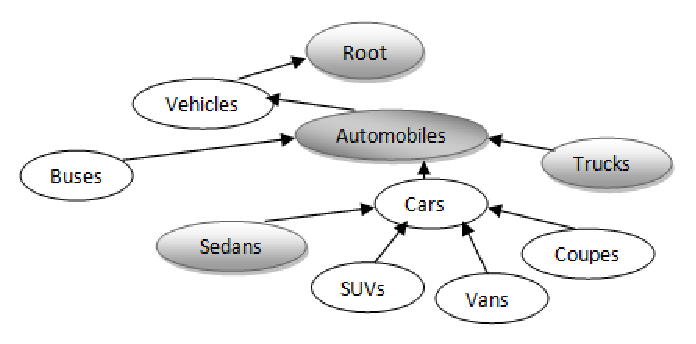
\includegraphics[width=85mm]{img/automotive_ontology.eps}
\caption{An abbreviated man-made automotive ontology - arrows represent inheritance relationships between the ontological classes.}
\label{fig:automotive_ontology}
\end{figure}

Suppose we want to find the category divergence between \textit{Sedans}
and \textit{Trucks} (Figure \ref{fig:automotive_ontology}). 
\textit{Sedans} is the subcategory of \textit{Cars}, and \textit{Trucks}
is the subcategory of \textit{Automobiles}. Therefore, the least common ancestor ($C$)
for these twoThis section presents ontology and copora, Query processing, ranking queries, and the query resolution mechanism. categories is \textit{Automobiles}. In addition, the tree height \textit{h = 4}.
So, the normalized divergence $cd$\textit{(Sedans, Trucks)} is \textit{7/12}
that is calculated from \textit{d(Sedans, Root) = 4}, \textit{d(Sedans, Automobiles) = 2}, and \textit{d(Trucks, Automobiles) = 1}.


\subsection{Executing} 

Once we have relevant QRMs through QRM ranking for a given user query, we can produce answers by re-running the pathways.

 The evaluation of this script by the QRE simulates the behavior of a human browsing the web, that is, clicking buttons to follow links, submitting forms, and highlighting of data to form a text answer.  The QRE assumes that becuase of the auto generated nature of deep web pages, the location of answers are the same irrespective of page changes.  It uses the relative XPath location to the answer node on HTML pages as described in \cite{Badica06}.


%When a user submits a new query to the Morpheus system, one or more stored QRMs are executed to obtain results. A QRM contains an XML script representing an algorithm that will obtain the required result. The evaluation of this script by the QRE simulates the behavior of a human browsing the web, that is, clicking buttons to follow links, submitting forms, highlighting data, cutting and pasting text, and constructing an answer in the form of a text string. There is greater complexity in dealing with web forms than with links. At present, the GET form submission method is used. This means that in preparation to submit a form, the Morpheus System builds a querystring consisting of name-value pairs. For a given form, there may be text fields, drop-down boxes, and among other components. In order to support form submission in such circumstances, the QRE performs different actions based upon the input type. For text fields, simply adding a key/value pair to the query string suffices. For a drop-down box, the QRE extracts the form element to find the appropriate value to include in the query string. It does this by examine each option in the drop-down and matching the user’s input to the text field in the option. The value attribute of the option is then added to the querystring. The value and text attributes of a dropdown option might be the same, but they are not guaranteed to be. All input data are kept in an internal table. The QRM script contains keys that allow the QRE to map SSQ inputs from the table to the appropriate form inputs. Furthermore, highlighted text segments collected during execution of the script are stored in the table. Once all actions in the script have been carried out, the QRE returns the textual answer this process has created. This answer is then be rendered in a browser displayed to the user.



% Results and conclusion  
\section{Results}
\label{sec:results}

% 3-4 queries 
% Human made ontology 
% Topic Models 

First, we built an ontology for the automotive realm exploiting the Wikipedia pages, categories, and WordNet synsets. For each of the classes in the ontolgy we built corpora from the corresponding Wikipedia pages. Figure \ref{fig:automotive_ontology} shows a subsection of this ontology.

 describes the question answering process for the user query, ``A 1997 Toyota Camry V6 needs what size tires?''


%% TODO - need to refer back to the table which is figure one.
%The Morpheus NLP engine parses this query into the constructs: WH:what, Descriptive Information:1997 Toyota Camry V6, Asking For:size tires. From the descriptive info, we generate the N-grams or terms 1997, 1997 Toyota, 1997 Toyota Camry,Toyota,Toyota Camry,Toyota Camry V6, Camry, Camry V6, and V6. For each of the terms, we determined relevant categories (non-increasing order of relevance) from the ontology corpora. Table \ref{tbl:term_categories} shows the top categories and their probabilities for each of the query term.
In Table \ref{tbl:nlp_engine_parse} we show the data that is output by the Morpheus NLP engines parse of the query .  It extracts the WH question


\begin{table}[h]\footnotesize
	\begin{tabular}{|l|p{4.2cm}|}
		\hline 
		WH & what \\
		\hline 
		Descriptive Information & 1997 Toyota Camry V6 \\
		\hline 
		Asking for & size tires \\
		\hline 
		ngrams & 1997, 1997 Toyota, 1997 Toyota Camry, Toyota, Toyota Camry, Toyota Camry V6, Camry, Camry V6, V6 \\
		\hline
	\end{tabular}
	\caption{The output of NLP engine parse}
	\label{tbl:nlp_engine_parse} 
\end{table}

\begin{table}[h]\footnotesize

\begin{tabular}{| p{3.2cm} | l | r |}
\hline 
Term & Category & $P(Category|Term)$ \\ \hline
1997 & Sedans & 404132.77e-14\\ 
1997 Toyota & Engines & 7.90e-14\\ 
Toyota  & Sedans & 3486670.15e-14\\ 
Toyota Camry & Sedans & 12147.23e-14\\ 
Toyota Camry V6 & Coupes & 13.80e-14\\ 
Camry & Sedans & 312034.20e-14\\ 
Camry V6 & Coupes & 13.80e-14\\ 
V6 & Sedans & 4464535.40e-14\\ \hline
\end{tabular}        

\caption{Terms' top categories and probabilities}
\label{tbl:term_categories}   

\end{table}

We found the top category of the terms in the candidate SSQ and determined the category divergence with the qualified SSQ classes in the QRM store. Then, we combined the divergence measure and
ranked QRMs based on the relevance score. Table \ref{tbl:ranked_queries} shows the top ranked SSQ for the query.  Finally, we execute the selected QRM and display the results to the user.

\begin{table}[h]\footnotesize

\begin{tabular}{| p{3.5cm} | p{3cm} | r |}
\hline
Query & Tagged Classes & Score\\ \hline
A 1997 Toyota Camry V6 needs what size tires? & IC:Sedans, Cars, Engines, Manufactures OC:size tires & 0.91\\ \hline 
What is the tire size for a 1998 Sienna XLE Van? & IC:Vans, Manufactures OC: tire size & 0.72\\ \hline 
%Where can I buy a headlight for a Toyota Camry V6? & IC:Manufactures, Sedans, Engines OC: where & - \\ \hline 
%What is the cost of a Toyota Camry V6 muffler? &  IC:Manufactures, Sedans, Engines OC: the clost  & 0.97 \\ \hline
\end{tabular}

\caption{Top ranked queries and relevance scores: IC - input classes, OC - output classes}
\label{tbl:ranked_queries}   

\end{table}


%\subsection{Discussion}
\section{Conclusion}

In this paper, we propose a novel question answering system that uses the deep web and previously answered user queries to answer similar questions. The system uses a path-finder to annotate answer paths so path-followers can discover answers to similar questions.  Each $(question, answer)$ pair is assigned a realm, and new questions are matched to the new $(question, answer)$ pairs. Classification of terms into classes is based on term frequency distributions in our corpora of web documents. We are investigating improvements to our solution by an approach similar to Topic Models \cite{Blei2003latentdirichlet}. 

Manually forming a corpus of wilipedia pages associated with a class is a cumbersome task. Topic Modeling provides a promising approach to identifying pages relevent to given class in a more automated manner.
%The Wikipedia page categories has limitations. Without supervision, the page categorization is often a challenging problem, because topics in the pages that belong to a realm (e.g. automotive) usually overlap. So we are evaluating the applicability of probabilistic topic models to web page categorization, and automatic generation of a realm-ontology based on the topics being extracted.
 


% 2. Current stage of the project 
% 3. Expected contribution to the topics of interest supported by iiWAS2010 




\section{Acknowledgments}

We thank Guillermo Cordero, Benjamin Landers, Patrick Meyer, Christopher Shields, and Terence Tai for their assistance building this system. This material is based upon work supported by the National Science Foundation under Grant No. 0712799 and a Graduate Research Fellowship to Christan Grant.

% Bibliography 
\bibliographystyle{abbrv}
\bibliography{morpheus}  


\end{document}
